Para a criação de um tarefa de aprendizado que seja capaz de verificar a autenticidade de assinaturas de indivíduos, é necessário primeiramente a existência de um conjunto de dados de imagens que possuam exemplos de assinaturas forjadas e genuínas, com o intuito de ser utilizado para o treinamento das CNNs. Para isto, utilizou-se os conjuntos de dados disponibilizados pela Competição de Verificação de Assinaturas de 2009 (SigComp2009, do inglês \emph{Signature Verification Competition}) realizado na Conferência Internacional em Análise e Reconhecimento de Documentos (ICDAR, do inglês \emph{International Conference on Document Analysis and Recognition}).

A SigComp2009 utilizou-se de conjuntos de dados diferentes em cada uma das duas etapa da competição. Para a etapa de treinamento, foi o utilizado o conjunto de assinaturas NISDCC, composto originalmente de 1920 assinaturas genuínas e forjadas, enquanto o conjunto coletado pelo \emph{Netherlands Forensic Institute} (NFI), foi utilizado para o processo de validação dos modelos submetidos na competição e composto por 1953 novas assinaturas genuínas e forjadas \cite{icdar2009}.

 % falar sobre a quantidade de assinaturas disponibilizada pelo site lá

% NISDCC: Norwegian Information Security laboratory and Donders Centre for Cognition
% NFI: Netherlands Forensic Institute

Os conjuntos disponibilizados pela SigComp2009 são composto por dois tipos de assinaturas, as assinaturas \emph{offline} e as assinaturas \emph{online}. Nas assinaturas \emph{offline}, é considerado apenas o aspecto estático da mesma, ou seja, uma imagem obtida após o processo da assinatura ter sido concluído. Os dados das assinaturas \emph{online}, por sua vez, contêm informações dinâmicas, que consistem em um arquivo de texto que descrevem os detalhes capturados em vários pontos durante o processo da assinatura, sendo estes as coordenadas $x$ e $y$ da ponta da caneta, a pressão exercida sobre a caneta, o ângulo de azimute e o ângulo de elevação \cite{icdar2009}.




\begin{figure}[h!]
\centering
\caption{Uma amostra das assinaturas \emph{offline} e \emph{online}. Font: \cite{icdar2009}}
\label{fig:sample-signature}
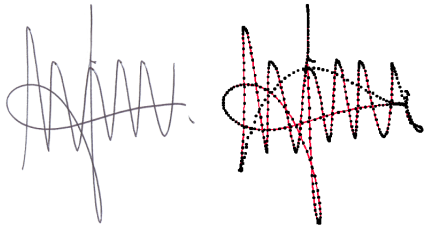
\includegraphics[width=0.5\textwidth]{imgs/sample-signature}
\end{figure}


% Conjuntos de treino e validação disponibilizados pela competição (NISDCC e NFI)
% Assinaturas online e offline
% Como foram feitas as assinaturas forjadas
% A quantidade de indivíduos no dataset
% A quantidade de assinaturas por indivíduo
